\documentclass{ws-ijait}

\usepackage[ruled, vlined]{algorithm2e}
\usepackage[T1]{fontenc}
\usepackage[utf8]{inputenc}
\usepackage[autostyle=false, style=english]{csquotes}
\usepackage[usenames,dvipsnames]{color}
\usepackage[justification=centering]{caption}
\usepackage[nodayofweek]{datetime}
\usepackage{amssymb}
\usepackage{booktabs}
\usepackage{balance}
% \usepackage{microtype}
\usepackage{enumitem}
\usepackage{graphicx}
\usepackage{gnuplottex}
\usepackage{pifont}
\usepackage{quoting}
\usepackage[hyphens]{url}
\usepackage{sepfootnotes}
\usepackage{setspace}
\usepackage[pdfpagelabels=false]{hyperref}
\usepackage{hypcap}

\newdateformat{lv}{\THEDAY{ }\shortmonthname[\THEMONTH] \THEYEAR}
\newcommand{\lastvisited}{Last visited \lv\today}

\MakeOuterQuote{"}
\newfootnotes{A}
\quotingsetup{vskip=0pt,font={itshape}}
\setenumerate{noitemsep,topsep=0pt,parsep=2pt,partopsep=0pt}
\setitemize{noitemsep,topsep=0pt,parsep=4pt,partopsep=0pt}
\setlength\floatsep{1.25\baselineskip plus 3pt minus 2pt}
\setlength\textfloatsep{1.25\baselineskip plus 3pt minus 2pt}
\setlength\intextsep{1.25\baselineskip plus 3pt minus 2 pt}
\def\algorithmautorefname{Algorithm}
\graphicspath{{img/}}
\newcommand{\cmark}{\ding{51}}
\newcommand{\xmark}{\ding{55}}

\newcommand\TODO[1]{\emph{\color{Red} TODO: #1}}
\renewcommand\comment[1]{\emph{\color{Gray}#1}}
\newcommand\code[1]{\texttt{#1}}
\newcommand\coderef[1]{\texttt{\ref{#1}}}
\newcommand\stringliteral[1]{\texttt{\char`\"#1\char`\"}}
\newcommand\len[1]{|#1|}
\newcommand\set[1]{\{#1\}}
\newcommand\surl[1]{\urlstyle{ff}\url{#1}}
\newcommand\Oof[1]{$\mathcal{O}(#1)$}

\begin{document}

\markboth{Vangelis Banos, Authors' Names}
{Instructions for Typing Manuscripts (Paper's Title)}

%%%%%%%%%%%%%%%%%%%%% Publisher's Area please ignore %%%%%%%%%%%%%%%
%
\catchline{}{}{}{}{}
%
%%%%%%%%%%%%%%%%%%%%%%%%%%%%%%%%%%%%%%%%%%%%%%%%%%%%%%%%%%%%%%%%%%%%

\title{INSTRUCTIONS FOR TYPESETTING MANUSCRIPTS\\
    USING \TeX\ OR \LaTeX\footnote{For the title, try not to use more than 
        3 lines. Typeset the title in 10 pt Times roman, uppercase and 
    boldface.}
}

\author{\footnotesize FIRST AUTHOR\footnote{
        Typeset names in 8~pt Times roman, uppercase. Use the footnote 
to indicate the present or permanent address of the author.}}

\address{University Department, University Name, Address\\
    City, State ZIP/Zone,
    Country\footnote{State completely without abbreviations, the
        affiliation and mailing address, including country. Typeset in 8~pt
    Times italic.}\\
first\_author@university.edu}

\author{SECOND AUTHOR}

\address{Group, Laboratory, Address\\
    City, State ZIP/Zone, Country\\
second\_author@group.com}

\maketitle

\begin{history}
    \received{(Day Month Year)}
    \revised{(Day Month Year)}
    \accepted{(Day Month Year)}
    %\comby{(xxxxxxxxxx)}
\end{history}

%\author{
  % 1st. author
%  \alignauthor
%	Vangelis Banos\\
%         \affaddr{Department of Informatics}\\
%         \affaddr{Aristotle University of Thessaloniki, Greece}\\
%         \email{\href{vmailto:vbanos@gmail.com}{vbanos@gmail.com}}
%  % 2nd. author
%	\alignauthor
%	Olivier Blanvillain\\
%         \affaddr{École Polytechnique Fédérale de Lausanne (EPFL)}\\
%         \affaddr{1015 Lausanne, Switzerland}\\
%         \email{\href{mailto:olivier.blanvillain@epfl.ch}{olivier.blanvillain@epfl.ch}}
  % 3rd. author
%	\alignauthor
%  Nikos Kasioumis\\
%         \affaddr{European Organization for Nuclear Research (CERN)}\\
%         \affaddr{1211 Geneva 23, Switzerland}\\
%         \email{\href{mailto:nikos.kasioumis@cern.ch}{nikos.kasioumis@cern.ch}}
%  \alignauthor
%	Yannis Manolopoulos\\
%         \affaddr{Department of Informatics}\\
%         \affaddr{Aristotle University of Thessaloniki, Greece}\\
%         \email{\href{vmailto:manolopo@csd.auth.gr}{manolopo@csd.auth.gr}}
%  }
%  
%  \additionalauthors{Yannis Manolopoulos (Department of Informatics, Aristotle University of Thessaloniki, Greece, {\texttt{manolopo@csd.auth.gr}})}
%  
%  \hypersetup{pageanchor=false}
  \maketitle

  \begin{abstract}
    Blogs are by nature a very dynamic and volatile communication medium. The BlogForever project aims on providing a generic platform for blog preservation, thus ensuring access to this information for future generations. This paper presents a key component of this archiving system: the web crawler. More precisely, our discussion will concentrate on techniques to automatically extract content, authors, dates and comments from blog posts. One of the main challenges in the preservation of web objects is the rapid evolution of technologies. For instance, the recent trend towards using JavaScript to dynamically generate pages on the client side constitutes a new obstacle for today's crawlers. We will show how we integrated a web browser into the harvesting process in order to address this issue. Furthermore, we will present a simple and robust algorithm to generate extraction rules based on string matching between a web feed and blog page contents. Our crawler will then use these rules throughout the blog, leading to a scalable extraction process.

  \end{abstract}
  
%  \category{H.3.3}{Information Storage and Retrieval}{Information Search and Retrieval}[Information filtering, Query formulation, Selection process]
%  \category{\\D.2.8}{Software Engineering}{Metrics}[Complexity measures, Performance measures]
  
  % In order of most significant, first letter of each word capitalized.
%  \terms{Design, Algorithms, Performance, Experimentation}

  % In alphabetical order, first letter of the first word capitalized.
  \keywords{Blog crawler, web data extraction, wrapper generation}

  \SetKw{Of}{of}
\SetKw{In}{in}
\SetKw{As}{as}
\SetKw{All}{all}
\SetKw{With}{with}
\SetKw{Over}{over}
\SetKw{Using}{for}
\SetKwFunction{Par}{}
\SetKwFunction{Rule}{Rule}
\SetKwFunction{Apply}{Apply}
\SetKwFunction{Bigram}{Bigram}
\SetKwFunction{AllRules}{\ref{allrulesAlgo}}
\SetKwFunction{Similarity}{\ref{similarityAlgo}}
\SetKwFunction{AbsolutePathTo}{AbsolutePathTo}

\DontPrintSemicolon
\SetProcNameSty{texttt}
\SetProcArgSty{textit}

\newcommand{\Arrow}{$\longleftarrow$~}
\newcommand{\Indent}{\hspace{12pt}}

\newcommand{\extractionAlgo}{
  \begin{algorithm}
    \caption{Best Extraction Rule}\label{extractionAlgo}
    \SetKwInOut{Input}{input}
    \SetKwInOut{Output}{output}
    \setstretch{1.1}
    \thinspace

    \Input{Set \emph{pageZipTarget} of Html and Text pairs}
    \Output{Best extraction rule}
    \BlankLine
    \emph{topRules \Arrow}new list\;
    \ForEach{\Par{page, target} \In pageZipTarget}{
      \emph{score \Arrow}new map\;
      \ForEach{rule \In \AllRules{page}}{
        \emph{extracted \Arrow \Apply{rule, page}}\;
        \emph{score \Of rule \Arrow \Similarity{extracted, target}}\;
      }
      \emph{topRules \Arrow topRules} + rule with highest \emph{score}\;
    }
    \Return{\emph{rule with highest occurrence in} topRules}\;
  \end{algorithm}
}

\newcommand{\allrulesAlgo}{
  \begin{function}
    \caption{AllRules(page)}\label{allrulesAlgo}
    \setstretch{1.1}

    \emph{rules} \Arrow new set\;
    \ForEach{node \In page}{
      \uIf{node \As \emph{\code{id} attribute}}{
        \emph{rules \Arrow rules} +\set{\stringliteral{
          //*[@id=`\textnormal{\it node.id}']}}\;
      } \ElseIf{node \As \emph{\code{class} attribute}}{
        \emph{rules \Arrow rules} +\set{\stringliteral{
          //*[@class=`\textnormal{\it node.class}']}}\;
      } \code{//} \lElse{
        \emph{rules \Arrow rules} +\set{\AbsolutePathTo{node}}%
        \comment{not sure if this commented else is usefull...}%
      }
    }
    \Return{rules}\;
  \end{function}
}

\newcommand{\similarityAlgo}{
  \begin{function}
    \caption{Similarity(string1, string2)}\label{similarityAlgo}
    \setstretch{1.1}

    \emph{bigrams1 \Arrow}set of pairs of adjacent characters in \emph{string1}\;
    \emph{bigrams2 \Arrow}set of pairs of adjacent characters in \emph{string2}\;
    \Return{\emph{2} \len{bigrams1 $\cap$ bigrams2} \emph{/} \Par{\len{bigrams1} \emph{+} \len{bigrams2}}}\;
    \end{function}
}

\newcommand{\linearAlgo}{
  \begin{algorithm}
    \caption{Linear Time Best Content Extraction Rule}\label{linearAlgo}
    \SetKwInOut{Input}{input}
    \SetKwInOut{Output}{output}
    \setstretch{1.1}
    \thinspace

    \Input{Set \emph{pageZipTarget} of Html and Text pairs}
    \Output{Best extraction rule}
    \BlankLine
    \emph{topRules \Arrow}new list\;
    \ForEach{\Par{page, target} \In pageZipTarget}{
      \emph{score \Arrow}new map\;
      \emph{bigrams \Arrow}new map\;
      \emph{bigrams \Of target \Arrow}set of pairs of adjacents in \emph{target}\;
      \ForEach{node \In page \With \emph{post-order traversal}}{
        \emph{bigrams \Of node \Arrow}
          \Par{\emph{set of pairs of adjacent chars}\;
          \Indent \In node.text $\bigcup$ bigrams \Of \All node.childs}\;
        \emph{score \Of node \Arrow }\;
          \Indent $\dfrac{ {2 \len{\Par{bigrams~\Of~node} \cap \Par{bigrams~\Of~target}}} }{ \len{bigrams~\Of~node} + \len{bigrams~\Of~target} }$\;
      }
      \emph{topRules \Arrow topRules} + \Rule{\emph{node with highest} score}\;
    }
    \Return{\emph{rule with highest occurrence in} topRules}\;
  \end{algorithm}
}

  \newcommand\similarityTable{
  \begin{table}[h]\centering
    \capstart
    \setstretch{1.1}
    \begin{tabular*}{\columnwidth}{
      @{}
      p{0.144\textwidth}
      p{0.18\textwidth}
      r
      r
      @{}
    }
    \toprule
    \emph{string1} & \emph{string2} & Dice & Leven. \\
    \midrule
    \stringliteral{Scheme Scala} & \stringliteral{Scala Scheme}
    & 90\% & 50\% \\
    \stringliteral{Rachid} & \stringliteral{Richard}
    & 18\% & 61\% \\
    \stringliteral{Rachid} & \stringliteral{Amy, Rachid and \newline all their friends}
    & 29\% & 31\% \\
    \bottomrule
    \end{tabular*}
  \caption{Examples of string similarities}\label{similarityTable}
  \end{table}
}

\newcommand\precisionTable{
  \begin{table}[h]\centering
    \capstart
    \setstretch{1.1}
    \setlength{\tabcolsep}{5pt}
    \begin{tabular*}{\columnwidth}{
      @{}
      l
      l
      p{0.204\columnwidth}
      p{0.18\columnwidth}
      r
      @{}
    }
    \toprule
    Target & Our~approach & Readability & Boilerpipe & Goose \\
    \midrule
    Article & 93.0\% & 88.1\% & 79.3\% & 79.2\% \\
    Title & 95.0\% & 74.0\% & N/A & 84.9\% \\
    \bottomrule
    \end{tabular*}
  \caption{Extraction success rates}\label{precisionTable}
  \end{table}
}

\newcommand\savevisualsTable{
  \cmark
  \xmark
  \begin{table}[h]\centering
    \capstart
    \setstretch{1.1}
    \setlength{\tabcolsep}{5pt}
    \begin{tabular*}{\columnwidth}{
      @{}
      l
      l
      p{0.204\columnwidth}
      p{0.18\columnwidth}
      r
      @{}
    }
    \toprule
    & GNU Wget  & wkhtmltopdf & OXPath & PhantomJS \\
    \midrule
    page interat  |   n    |      n      |   y    |    y
    js support    |   n    |      y      |   y    |    y
    running time  | 0.50s  |    7.58s    | 22.04s |  3.32s

    Article & 93.0\% & 88.1\% & 79.3\% & 79.2\% \\
    Title & 95.0\% & 74.0\% & N/A & 84.9\% \\
    \bottomrule
    \end{tabular*}
  \caption{Extraction success rates}\label{savevisualsTable}
  \end{table}
}

  ~\\~\\~\\~\\~\\~\\~\\
  \section{Intro}

Aims and contributions of this work. Example from my last paper to see the format:
\surl{http://purl.pt/24107/1/iPres2013_PDF/CLEAR\%20a\%20credible\%20method\%20to\%20evaluate\%20website\%20archivability.pdf}

\begin{enumerate}
  \item Introduce the importance for blog preservation
  \item Explain the difficulties in harvesting blogs
  \item Explain why open source and Invenio
  \item Introduce the blog crawler
\end{enumerate}

Challenges consist of:
\begin{enumerate}
  \item Providing a high degree of automation
  \item Dealing with large volumes of data
\end{enumerate}

Semi-structured nature of Web pages

Labeled ordered rooted trees
XML Path Language(XPath)

  \section{Related work}
2-related-work.tex

Web Object Identification for Web Automation and Meta-Search,
\\
http://www.dbai.tuwien.ac.at/proj/ta\\
mcrow/download/Kordomatis2013WIMS.pdf

Self-supervised Automated Wrapper Generation for Weblog Data Extraction,
\\
https://github.com/OlivierBlanvillai\\
n/blogforever-crawler-publication/raw\\
/master/papers/bncod\_published.pdf

Web Data Extraction, Applications and Techniques: A Survey,
\\
http://www.emilio.ferrara.name/wp-co\\
ntent/uploads/2011/07/survey-csur.pdf

Archiving Data Objects using Web Feeds,
\\
http://hal.archives-ouvertes.fr/docs\\
/00/53/79/62/PDF/iwawienna.pdf

Intelligent and Adaptive Crawling of Web Applications for Web Archiving,
\\
http://pierre.senellart.com/publicat\\
ions/faheem2013intelligent.pdf

Zero-cost Labelling with Web Feeds for Weblog Data Extraction,
\\
http://www2013.org/companion/p73.pdf\\


OXPath: A Language for Scalable, Memory-efficient Data Extraction from Web Applications,
\\
http://www.vldb.org/pvldb/vol4/p1016-furche.pdf

  \section{Algorithms}\label{algorithms}

This section explains in detail the algorithms we developed to extract blog posts' content and its variations for authors, dates and comments.
We explain how we take advantage of blog specific characteristics to build extraction rules applicable to all posts of a blog.
Our focus is on minimising the algorithmic complexity while keeping our approach simple and generic.

%%%%%%%%%%%%%%%%%%%%%%%
\subsection{Motivation}
% html extraction is not trival
Extracting metadata and content from HTML documents is a challenging task. Standards and format recommendations have been around for quite some time, strictly specifying how HTML documents should be organised \TODO{ref to W3C standards}.
For instance the \code{<h1></h1>} tags should contain the highest-level heading of the page and must not appear more than once per page\cite{w3c2002}.
More recently, specifications such as Microdata\cite{whatwg2013} define ways to embed semantic information and metadata inside HTML documents, but these still suffer from very low usage: estimated to be used in less than 0.5\%\cite{andrewrogers2013} of websites. In fact, the majority of websites rely on the generic \code{<span></span>} and \code{<div></div>} container elements with custom \code{id} or \code{class} attributes to organise structure pages\cite{brianwilson2008}\TODO{FIX REF!}, and more than 95\% of pages do not pass HTML validation\cite{brianwilson2008-a}. Under such circumstances, relying on HTML structure to extract content from web pages is not viable and other techniques need to be employed.

\TODO{Assumption is not a good word, we are based on facts from previous work.
I suggest that you restructure this part as follows:

Having blogs as our target websites, we are taking into account  the following facts that play a central role in the extraction process.

1. "Blog is a kind of web page [with] frequent, usually brief posts, with the immediacy of reverse chronological order" (+ ref to BlogForever D2.2: BlogForever Data Model 
https://zenodo.org/record/7488/files/BlogForever\_D2\_2WeblogDataModel.pdf 

2. blogs provide web feeds: structured and standardised views of the most recent blog posts.

3. Web feeds contain information regarding the latest blog posts (usually 10 or 20 entries) + ref

4. posts of the same blog share a similar HTML structure.

Consequently, in order to effectively archive old blog content, it is necessary to download and process pages beyond the ones referenced in web feeds.
}

\Anotecontent{assumptions}{Our experiments on a large dataset of blogs showed that failing tests were either due to a violation of one of these assumptions, or to an insufficient amount of text in posts, such as \emph{photoblogs} with short captions.}

% assumptions when working with blogs
Having blogs as our target websites, the assumptions we made and which play a central role in the extraction process are the following\Anote{assumptions}:
\begin{enumerate}[label={(\arabic*)}]
  \item\label{havefeedAssum} Blogs provide web feeds: structured and standardized views of the most recent posts of a blog,\TODO{mention RSS and Atom, just to confirm to the reader what a web feed is?}
  \item\label{similarhtmlAssum} Posts of the same blog share a similar HTML structure.
\end{enumerate}
Web feeds usually contain about 20 posts\cite{oita2010},\TODO{Add more info on web feeds, merge with the text on intro.} often less than the total number of posts in blogs. Consequently, in order to effectively archive old content from blogs, it is necessary to download and process pages beyond the ones referenced in the feed.

%%%%%%%%%%%%%%%%%%%%%%%%%%%%%%%
\subsection{Content extraction}
\TODO{When I read this section for the first time, I was confused.
After I also read 3.3 and 3.4 I understood better.
You should have a nicely structured overview of the algorithm in 3.2 and have references for 3.3 and 3.4
When you describe the algorithm overview, you should say explicitly that function X and operation Y is explained in section Z, etc}
% per blog procedure, related work
To extract content, authors, dates and comments from blog posts, we started by building extraction rules from the data given in the blog's web feed. \TODO{These rules take advantaged of the facts presented in 3.1 to create a more efficient data extraction process, outperforming more generic extraction algorithms that work directly with HTML pages.}These rules take advantage of our assumption that the HTML structure between different posts of the same blog is the same, in order to be applicable to all the posts of a blog. This approach has been examined in the past and has demonstrated great results (see \cite{gkotsis2013}, \cite{oita2010}), outperforming more generic extraction algorithms that work directly on HTML pages.\comment{This might be a bit too raw, give more context at this point?}

\extractionAlgo

% algorithm, inputs/output
Algorithm \ref{extractionAlgo} shows the steps we follow to build extraction rules for the content of blog posts. As input, it takes a set of pairs of HTML pages and target contents, and finally returns an extraction rule. This rule is such that when applied to other input pages, the extracted contents are as similar as possible to the corresponding target contents.

% general idea, embarrassingly parallel
The idea is quite simple: to compute the best extraction rule for each pair of HTML pages and target content and to finally return the most frequent best rule. Making each of these computations independent might seem like a loss of information compared to alternative solutions such as having a global score for each rule, computed as the average of each rule's score over all the pages of the feed. In our experimentation we observed several cases where the independent solution performs better\TODO{example, reference or proof?}. When web feeds have posts with very short content, mean based solutions tend to be more influenced by these outliers and are inclined to return erroneous rules which fail to return target contents but constantly have an average score.\TODO{rephrase!}

In addition, having an independent computation for each input makes the algorithm \emph{embarrassingly parallel}\comment{it's a coined term, so it's fine, but should we have a reference here? -> Can't find a good one..}: iterations of the outer loop can trivially be executed by multiple threads.

% input from assumptions.
Before going into further details about annex functions and time complexity, we should explain how the previously stated assumptions relate to Algorithm \ref{extractionAlgo}. Given a blog, assumption \ref{havefeedAssum} allows the crawler to obtain input for the algorithm. Indeed, web feeds provide either textual content or descriptions for their entries, as well as links to the corresponding pages. Assumption \ref{similarhtmlAssum} guarantees the existence of an appropriate extraction rule, as well as its applicability to all the posts of a blog.


%%%%%%%%%%%%%%%%%%%%%%%%%%%%%%%%%%%%%%%%%%%%%%%%%%%
\subsection{Extraction rules and string similarity}
% xpath selectors (id, else class, else path)
In our implementation, rules are queries in the XML Path Language (XPath). Consequently, standard libraries can be used to parse HTML pages and apply extraction rules, thus providing the \code{Apply} function, used in Algorithm \ref{extractionAlgo}. We experimented with 3 types of XPath queries: selection over the HTML \code{id} attribute, selection over the HTML \code{class} attribute and selection with the absolute path in the HTML tree. \code{id} attributes are expected to be unique, and \code{class} attributes have showed to have better blog consistency than absolute paths. For these reasons, the \coderef{allrulesAlgo} function only returns the best rule for each node:

\allrulesAlgo

% string similarity
Unsurprisingly, the choice of the string similarity algorithm greatly influences the running time and precision of the extraction process. We chose the Sørensen–Dice coefficient similarity\cite{dice1945}, which, to the best of our knowledge\comment{maybe remove this? it weakens our choice a bit. -> at the same time it might not be the only one...}, is the only string similarity algorithm fulfilling the following criteria:

\begin{enumerate}
  \item\label{wordorderProp} Has low sensitivity to word ordering
  \item\label{lengthProp} Has low sensitivity to length variations
  \item\label{linearProp} Runs in linear time
\end{enumerate}

Properties \ref{wordorderProp} and \ref{lengthProp} are essential to deal with cases where a blog's web feed only contains an abstract or a subset of the entire post content. Table \ref{similarityTable} gives examples to illustrate how these two properties are fulfilled by the Sørensen–Dice coefficient similarity but do not hold for \emph{edit distance} based similarities such as the Levenshtein\cite{levenshtein1966} similarity.

\similarityTable

The Sørensen–Dice coefficient method operates by first building sets of pairs of adjacent characters, also knows as \emph{bigrams}, and then applying the \emph{quotient of similarity} formula:

\TODO{similatiry -> score function}
\similarityAlgo

%%%%%%%%%%%%%%%%%%%%%%%%%%%%%%%%%%%%%%%%%%%%%%%%%%%%%
\subsection{Time complexity and linear reformulation}
% algo 1 is quadratic
With both the \coderef{allrulesAlgo} and \coderef{similarityAlgo} functions defined, we will show that Algorithm \ref{extractionAlgo} has a quadratic running time. First, let's assume that we have at our disposal a linear time HTML parser that constructs an appropriate data structure indexing HTML nodes on their \code{id} and \code{class} attributes, effectively making \code{Apply}~$\in$~\Oof{1}. As stated before the outer loop splits the input into independent computations and each call to \coderef{allrulesAlgo} returns (in linear time) at most as many rules as the number of nodes in its \emph{page} argument. Therefore, the body of the inner loop will be executed \Oof{n} times. Because the extraction rule can return any subtree of the queried page, each call to \coderef{similarityAlgo} takes \Oof{n}, leading to an overall quadratic running time.

% Linear reformulation
We will now present Algorithm \ref{linearAlgo}, a dynamic programming reformulation of Algorithm \ref{extractionAlgo} with linear running time. While very intuitive, the original idea of first generating extraction rules and then picking these best rules prevents us from an effective reuse of previously computed bigrams. For instance, when evaluating the extraction rule for the HTML root node, Algorithm \ref{extractionAlgo} will obtain the complete string of the page and pass it to the \coderef{similarityAlgo} function. At this point, the information on where the string could be split into substrings with already computed bigrams is not accessible, and the bigrams of the page have to be computed by linearly traversing the entire string. To overcome this limitation and implement $memoization$ \comment{without R!}over the bigram computations, Algorithm \ref{linearAlgo} uses a post-order traversal of the HTML tree to compute node bigrams from their children bigrams. This way we avoid serializing HTML subtrees for each bigram computation and we can guarantee that each character of the HTML page will be read at most once during the bigrams computation. Thus, the cumulated time needed to compute bigrams of \emph{node.text} is linear.

\linearAlgo

% End of proof
To conclude the proof that algorithm \ref{linearAlgo} runs in linear time we show that all its inner loop computations other than bigrams of \emph{node.text} can be done in constant \emph{amortized} time. As the number of edges in a tree is one less than the number of nodes, the \emph{amortised} number of bigram unions per inner loop iteration is one. Each \emph{quotient of similarity} computation requires one bigram intersection and three bigram length computations. Over a finite alphabet (we used printable ASCII), bigram sizes have bounded size and each of these operations can be done in constant time.

%%%%%%%%%%%%%%%%%%%%%%%%%%%%%%%%%%%%%%%%%%%%%%%%%%%%%%%
\subsection{Variations for authors, dates and comments}
% Intro
In the current state algorithms \ref{extractionAlgo} and \ref{linearAlgo} will perform poorly for author and date extraction and are not suitable for comment extraction. This subsection presents variations on the general extraction techniques presented before. \TODO{Rephrase this to say that we don't show the full algos because it's just as in the 2 previous with customised score function!}Due to space constraints, we will only provide the main ideas and omit algorithmic and implementation details.

% Authors
The case of authors is problematic because it is not uncommon to encounter the author's name at several places in a page, leading to several rules with maximum score. The heuristic we use to get around this issue consists of adding a new component in the scores of authors extraction rules: the \emph{tree distance} between the evaluated node and the post content node. This new score component takes advantage of the positioning of post's authors which often is a direct child or shares its parent with the post content node.

% Dates, authors
Dates are affected by the same duplication issue, as well as the inconsistence of format between web feeds and web pages. Our solution is to use multiple \emph{target} strings, while extending the rule that we previously described for author extraction. For instance, if the feed indicates that a post was published on
\stringliteral{Thu, 01 Jan 1970 00:00:00}, our algorithm will create a rule that extracts one of \stringliteral{Thursday January 1, 1970}, \stringliteral{1970-01-01}, \stringliteral{43 years ago} and so on. We use a list of \TODO{none so far :(} target date formats that was empirically built during our experiments. While this list is certainly not exhaustive, our approach using string similarity on multiple target dates is robust and tolerant to format variations. We do not, so far, support dates in multiple languages but English was sufficient for our experiments.

% Comments
Comments are usually available in separate web feeds, one per blog post. Similarly to blog feeds, comment feeds have a limited number of entries, and in case a blog post has more comments than the ones appearing in the feed, comments have to be extracted from the post web page. To do so we use algorithm \ref{extractionAlgo} with the following modifications:
\begin{enumerate}
  \item Rules that return less HTML nodes than the number of comments on the feed are filtered out.
  \item The score of a rule is the value of the \emph{maximum weighted matching} in the \emph{complete bipartite graph} $G = (U, V, E)$, where $U$ is the set of HTML nodes returned by the rule, $V$ is the set of target comment fields from the web feed (such as comment authors) and $E(u, v)$ as weight equal to \code{\ref{similarityAlgo}(}$u, v$\code{)}.
\end{enumerate}
Our crawler executes this algorithm on each post that present a comment feed overflow, thus supporting blogs with multiple commenting engines. Comment contents are extracted first, which allows to narrow down the first modification by fixing a target number of comments.

  \section{Architecture}
\label{architecture}

We present the BlogForever crawler system architecture which implements 
the proposed algorithms for weblog data extraction via the generation 
of extraction rules. We describe the system architecture and discuss 
the software tools and techniques we used, such as the enrichment of the 
Scrapy framework for our specific usage and the integration of a headless 
web browser into the harvesting process to achieve content extraction 
from webpages which use JavaScript to display content. Following, 
we focus on the scalability design and distributed architecture of our 
system. Finally, we present our provisions for interoperability using 
established open standards which increases the value and reusability 
of the proposed system in many contexts. 

%%%%%%%%%%%%%%%%%%%%%%%%%
\subsection{System and workflow}

The BlogForever crawler is a Python\footnote{\label{python}\url{http://www.python.org/}} 
application which is based on  Scrapy, an open-source framework for web crawling. 
Scrapy provides an elegant and modular architecture illustrated 
in Fig. \ref{scrapyarchitecture}. Several components can be plugged into 
the Scrapy core infrastructure. Following, we present each part of the 
architecture and our own contributions:

\begin{itemize}
\item 
\emph{Spiders} define how a target website is scraped, including how to 
perform the crawl (i.e. follow links). The BlogForever crawer implementation
includes two new types of spiders: \emph{NewCrawl} and \emph{UpdateCrawl},
which implement the logic to respectively crawl a new blog and get updates
from a previously crawled blog.
\item 
\emph{Item Pipeline} defines the processing of extracted data from 
the spiders through several components that are executed sequentially. 
The BlogForever crawler implementation includes a new item pipeline 
which orchestrates all aspects of crawling. More specifically the 
BlogForever pipeline is defined as follows:
  \begin{enumerate}
  \item JavaScript rendering,
  \item Extract content,
  \item Extract comments,
  \item Download multimedia files,
  \item Prepare Archival Information Packages (APIs) to propagate 
the results to potential back-ends.
  \end{enumerate}
\item 
\emph{Downloader Middlewares} is a framework of hooks into Scrapy’s 
request/response processing and altering Scrapy’s requests and responses. 
\item 
\emph{Spider Middlewares} is a framework of hooks into Scrapy’s spider 
processing mechanism.
\end{itemize}

\begin{figure}[t]
\capstart
\centering
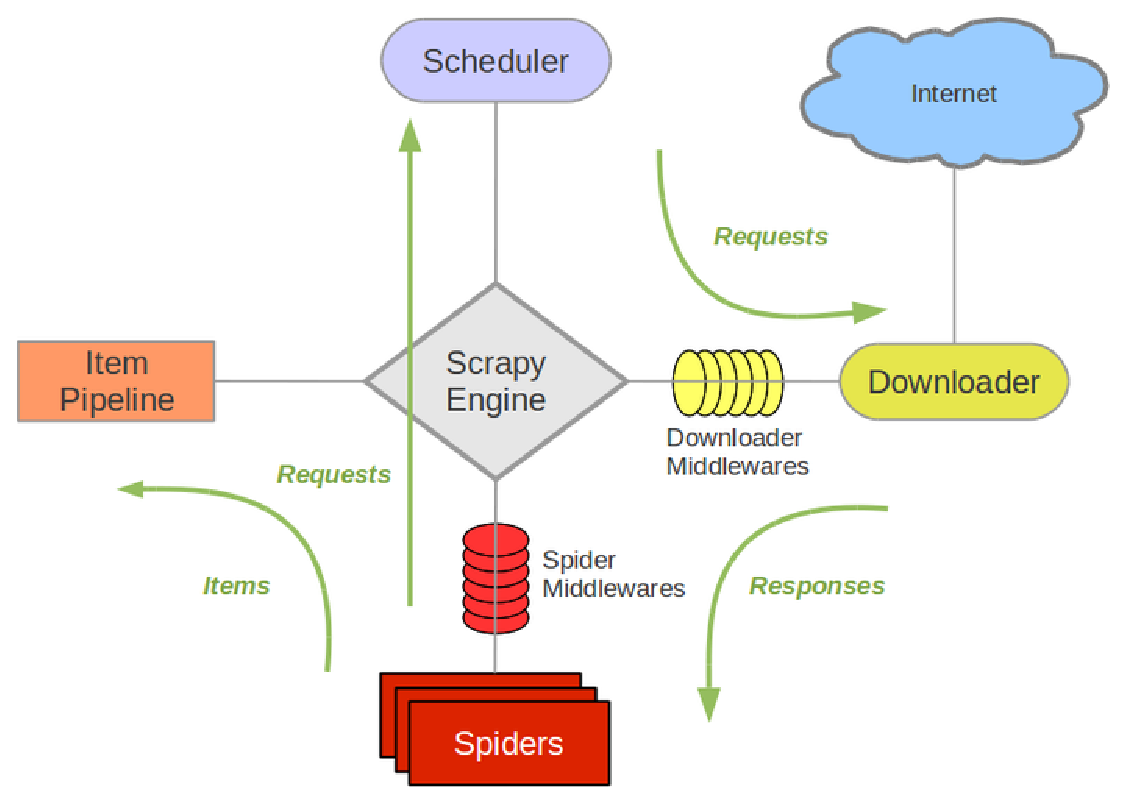
\includegraphics[width=\textwidth]{./img/scrapy_architecture.eps}
\caption{Overview of the crawler architecture. (Credit: Pablo Hoffman, Daniel Graña, Scrapy)}
\label{scrapyarchitecture}
\end{figure}

The system architecture providers great modularity. This is illustrated 
clearly in our work with the following
example:

\begin{itemize}
\item 
If it is necessary to disable JavaScript rendering or plugging in an 
alternative back-end can be done by editing a single line of code. 
\item The features to extract comments and download multimedia files 
were implemented after creating the initial logic to extract content 
and were added as extra steps in the pipeline.
\item The requirement to implement interoperability provisions later 
presented in section \ref{interop} was easily covered with the implementation 
of an extra middleware plugin which was invoked from the main crawler 
architecture. No further modifications were necessary in the code.
\end{itemize}


In the remaining parts of this section, we elaborate our work on each 
specific part of the crawler system.

%%%%%%%%%%%%%%%%%%%%%%%%%%%%%%%%%
\subsection{JavaScript rendering}

JavaScript is a widely used language for client-side scripting. 
While some applications simply use it for aesthetics, an increasing 
number of websites use JavaScript to download and display content. 
In such cases, traditional HTML based crawlers do not see web pages 
as they are presented to a human visitor by a web browser, and might 
therefore be obsolete for data extraction.

In our experiments whilst crawling the blogosphere, we encountered 
several blogs where crawled data was incomplete because of the lack 
of JavaScript interpretation. The most frequent cases were blogs using 
the Disqus\footnote{\url{http://disqus.com/websites}} and 
LiveFyre\footnote{\url{http://web.livefyre.com}} comment hosting services. 
For webmasters, these tools are very handy because the entire comments 
infrastructure is externalized and their setup essentially comes down 
to including a JavaScript snippet in each target page. Both of these 
services heavily rely on JavaScript to download and display the comments, 
even providing functionalities such as real-time updates for edits and 
newly written comments. Less commonly, some blogs are fully rendered 
using JavaScript. When loading such websites, the web browser will not 
receive the page content as an HTML document, but will instead have 
to execute JavaScript code to download and display the page content. 
The Blogger platform provides the \emph{Dynamic Views} as a default 
template, which uses this mechanism~\cite{antinharasymiv2011}.

To support blogs with JavaScript-generated content, we embed a full web 
browser into the crawler. After considering multiple options, we opted 
for PhantomJS\footnote{\url{http://phantomjs.org}}, a headless web 
browser with great performance and scripting capabilities. The JavaScript 
rendering is the very first step of web page processing. Therefore, 
extracting blog post articles, comments or multimedia files works equally 
well on blogs with JavaScript-generated content and on traditional 
HTML-only blogs.

When the number of comments on a page exceeds a certain threshold, both 
Disqus and LiveFyre will only load the most recent ones and the stream 
of comments will end with a \emph{Show More Comments} button. As part of 
the page loading process, we instruct PhantomJS to repeatedly click on 
these buttons until all comments are loaded. Paths to Disqus and LiveFyre 
\emph{Show More} buttons are manually obtained. They constitute the 
only non-generic elements of our extraction stack which require human 
intervention to maintain and extend to other commenting platforms.

%%%%%%%%%%%%%%%%%%%%%%%%%%%%%
\subsection{Content extraction}\label{enrichingscrapy}

In order to identify web pages as blog posts, our implementation enriches 
Scrapy with two components to narrow the extraction process down to the 
subsets of pages which are blog posts: \emph{blog post identification} 
and \emph{download priority heuristic}.

Given a URL entry point to a website, the default Scrapy behaviour 
traverses all the pages of the same domain in a \emph{last-in-first-out} 
manner. The \emph{blog post identification} function is able to identify 
whether an URL points to a blog post or not. Internally, for each blog, 
this function uses a regular expression constructed from the blog post 
URLs found in the web feed. This simple approach requires that blogs use 
the same URL pattern for all their posts (or false negatives will occur) 
which has to be distinct for pages that are not posts (or false positives 
will occur). In practice, this assumption holds for all blog platforms 
we encountered and seems to be a common practice among web developers.

In order to efficiently deal with blogs that have a large number of 
pages which are not posts, the \emph{blog post identification} mechanism 
is not sufficient. Indeed, after all pages identified as blog posts 
are processed, the crawler needs to download all other pages to search 
for additional blog posts. To replace the naive \emph{random walk}, 
\emph{depth first search} or \emph{breadth first search} web site 
traversals, we use a priority queue where priorities for new URLs are 
determined by a machine learning system. This mechanism has shown 
to be mandatory for blogs hosted on a single domain alongside large 
number of other types of web pages, such as those in forums or wikis.

The idea is to give high priority to URLs which are believed to 
point to pages with links to blog posts. These predictions are 
done using an active \emph{Distance-Weighted $k$-Nearest-Neighbour} 
classifier~\cite{dudani1976}. Let $L(u)$ be the number of links to blog 
posts contained in a page with URL $u$. Whenever a page is downloaded, 
its URL $u$ and $L(u)$ are given to the machine learning system as 
training data. When the crawler encounters a new URL $v$, it will ask the 
machine learning system for an estimation of $L(v)$, and use this value 
as the download priority of $v$. $L(v)$ is estimated by calculating a 
weighted average of the values of the $k$ URLs most similar to $v$.

%%%%%%%%%%%%%%%%%%%%%%%%%%%%%
\subsection{The BlogForever metadata schema for interoperability}
\label{interop}

One of the key BlogForever project goals is interoperability with third 
party platforms. The original BlogForever crawler was intended to
insert blog data directly to the BlogForever repository component but
later the architecture was reworked to make it possible to use
other storage and archiving systems as well. 
To achieve this goal, we implement a special interoperability middleware 
for the spider to produce Archival Information Packages (AIPs) from 
harvested blog content. The AIPs can be used by any software platform 
which complies with the OAIS reference model~\cite{lavoie2000meeting}. 
It must be noted also that this is the first time weblog content is 
encoded in this way.

The AIPs consist of XML files structured using the 
METS~\cite{cantara2005mets} standard for encoding metadata and 
content. METS is widely adopted and supported by all popular digital 
library systems. In addition, the blog content attributes which 
are included in the METS XML packages are encoded using the MARCXML
Schema\cite{marc2003official}. The reason for the selection of MARCXML 
is the wide adoption of the standard, its flexibility and extensibility, 
as well as previous experience with the Invenio digital library
system\footnote{\url{http://invenio-software.org/}} which is also based
on MARCXML.

There are three kinds of entities which can be included in an AIP: 
Blog, Entry and Comment. The content extracted from weblogs is mapped 
to the relevant entities using the following rule: If an attribute is 
already defined in MARC for other content types use the same MARC code 
for blogs. If an attribute is totally new, an unused MARC 9xx tag is 
chosen to represent it, composing therefore the BlogForever metadata 
schema~\cite{llopis2012d4}. Following, we present the BlogForever 
metadata schema for Blog, Post, Page and Comment entities in Tables 
\ref{table:blog-record-attributes}, 
\ref{table:post-page-shared-attributes} and 
\ref{table:comment-attributes}.

\begin{table}
\tbl{Blog record attributes - MARC 21 representations mapping.}
{\begin{tabular}{@{}ll@{}} \toprule
\textbf{Blog attribute} & \textbf{MARC 21 representation} \\ \hline
title & 245 \$a \\
subtitle & 245 \$b \\
URI & 520 \$u\\
aliases & 100 \$g \\
status\_code & 952 \$a\\
language & 041 \$a\\
encoding & 532\\
sitemap\_uri & 520\\
platform & 781 \$a\\
platform\_version & 781 \$b\\
webmaster & 955 \$a\\
hosting\_ip & 956 \$a\\
location\_city & 270 \$d\\
location\_country & 270 \$b\\
last\_activity\_date & 954 \$a\\
post\_frequency & 954 \$b\\
update\_frequency & 954 \$c\\
copyright & 542\\
ownership\_rights & 542\\
distribution\_rights & 542\\
access\_rights & 542\\
license & 542 \$f\\ \hline
\end{tabular}}
\label{table:blog-record-attributes}
\end{table}

\begin{table}
\tbl{Blog record attributes - MARC 21 representations mapping.}
{\begin{tabular}{@{}ll@{}} \toprule
\textbf{Post and page attribute} & \textbf{MARC 21 representation} \\ \hline
title & 245 \$a \\
subtitle & 245 \$b \\
full\_content & 520 \$a \\
full\_content\_format & 520 \$b \\
author & 100 \$a \\
URI & 520 \$u \\
aliases & 100 \$g \\
alt\_identifier (UR) & 0247 \$a \\
date\_created & 269 \$c\\
date\_modified & 260 \$m \\
version & 950 \$a \\
status\_code & 952 \$a \\
response\_code & 952 \$b \\
geo\_longitude & 342 \$g \\
geo\_latitude & 342 \$h \\
access\_restriction & 506 \\
has\_reply & 788 \$a \\
last\_reply\_date & 788 \$c \\
num\_of\_replies & 788 \$b \\
child\_of & 760 \$o \$4 \$w\\
\hline
\end{tabular}}
\label{table:post-page-shared-attributes}
\end{table}

\begin{table}
\tbl{Comment record attributes - MARC tags mapping.}
{\begin{tabular}{@{}ll@{}} \toprule
\textbf{Comment attribute} & \textbf{MARC 21 representation} \\ \hline
subject & 245 \$a\\
author & 100 \$a \\
full\_content & 520 \$a \\
full\_content\_format & 520 \$b \\
URI & 520 \$u\\
status & 952 \$a\\
date\_added & 269 \$c\\
date\_modified & 269 \$m\\
addressed\_to\_URI & 789 \$u\\
%& \textit{timezone} & \\
%& \textit{format} & \\
%& comment\_type (UR) & \\
%& source\_URI (UR) & \\
%& source\_name (UR) & \\
geo\_longitude & 342 \$g \\
geo\_latitude & 342 \$h \\
has\_reply & 788 \$a \\
num\_replies & 788 \$b\\
is\_child\_of\_post & 773 \$o \$4 \$w\\
is\_child\_of\_comment & 773 \$o \$4 \$w\\ \hline
\end{tabular}}
\label{table:comment-attributes}
\end{table}

%%%%%%%%%%%%%%%%%%%%%%%%
\subsection{Distributed architecture and scalability}
\label{scalability}

One of the problems of web crawling is the large amount 
of input which need to be processed. To address this issue, 
it is crucial to build every layer of the system with scalability in 
mind~\cite{thereactivemanifesto2013}. 

The BlogForever Crawler, and in particular the two core procedures 
\emph{NewCrawl} and \emph{UpdateCrawl}, are designed to be usable as 
part of an event-driven, scalable and fault-resilient distributed system. 
Heading in this direction, we made the key design choice to have 
both \emph{NewCrawl} and \emph{UpdateCrawl} as stateless components. 
From a high-level point of view, these two components are \emph{purely functional}:
%
\begin{eqnarray*}
NewCrawl:    &~ URL \rightarrow \mathcal{P}(RECORD) \\
UpdateCrawl: &~ URL \times DATE \rightarrow \mathcal{P}(RECORD)
\end{eqnarray*}
%
where $URL$, $DATE$ and $RECORD$ are respectively the set of all URLs, 
dates and records, and $\mathcal{P}$ designates the power set operator. 
By delegating all shared mutable state to the back-end system, 
web crawler instances can be added, removed and used interchangeably.

To implement a distributed crawler architecture, we choose to use 
Scrapyd\footnote{\url{http://scrapyd.readthedocs.org/en/latest/}}, 
an application for deploying and running Scrapy spiders. 
The process is quite straightforward:

\begin{enumerate}
\item 
Deploy the BlogForever crawler in any number of servers according 
to requirements. Using the Scrapyd component which is run as a system 
daemon, each crawler is listening for requests to run crawling tasks 
and spawn a process for each new command.
\item 
Implement a small control program that reads the list of target weblogs 
which need to be crawled and issue commands in a round-robin fashion 
using the Scrapyd JSON 
API\footnote{\url{http://scrapyd.readthedocs.org/en/latest/api.html}}. 
\item 
All crawlers share a common storage service where they save the crawling 
results. 
\end{enumerate}


  \section{Evaluation}\label{evaluation}

Our evaluation is articulated in two parts. First, we compare the article extraction procedure presented in \autoref{algorithms} with three open-source projects capable of extracting article and title from web pages. The comparison will show that our blog-targeted solution has better performance both in terms of success rate and running time. Second, a discussion is held regarding the different solutions available to archive data beyond what is available in the HTML source code. Extraction of authors, dates and comments is not part of this evaluation because of the lack of publicly available competing projects and reference data sets.

In our experiments we used \emph{Debian GNU/Linux 7.2}, \emph{Python 2.7} and an \emph{Intel Core i7-3770 3.4 GHz} processor. Timing measurements were made on a single dedicated core with garbage collection disabled. The Git repository for this paper \cite{repositoryofthispaper} contains the necessary scripts and instructions to reproduce all the evaluation experiments presented in this section. The crawler source code is available under the MIT license from the project's websites \cite{blogforevercrawler}.

%%%%%%%%%%%%%%%%%%%%%%%%%%%%%%%%%%%%%
\subsection{Extraction success rates}
To evaluate article and title extraction from blog posts we compared our approach to three open source projects: Readability \cite{python-readability2011}, Boilerpipe \cite{kohlschuetter2010} and Goose \cite{goose2012}, implemented in JavaScript, Java and Scala respectively. These projects are more generic than our blog-specific approach in the sense that they are able to identify and extract data directly from HTML source code, and do not make use of web feeds or structural similarities between pages of the same blog (observations \ref{havefeedAssum} and \ref{similarhtmlAssum}). \autoref{precisionTable} shows the extraction success rates for article and title on a test sample of 2300 blog posts obtained from the Spinn3r dataset \cite{burton2011}.

% An extraction was considered successful when the returned string is a least 0.5 similar to the reference string, with respect to the Sørensen–Dice coefficient similarity.

\precisionTable

On our test dataset \autoref{extractionAlgo} outperformed the competition by 4.9\% on article extraction and 10.1\% on title extraction. It is important to stress that Readability, Boilerpipe and Goose rely on generic techniques such as word density, paragraph clustering and heuristics on HTML tagging conventions, which are designed to work for any type of web page. On the contrary, our algorithm is only suitable for pages with associated web feeds, as these provide the reference data used to build extraction rules. Therefore, results showen in \autoref{precisionTable} should not be interpreted as a general quality evaluation of the different projects, but simply as an evidence that our approach is more suitable when working with blogs.


%%%%%%%%%%%%%%%%%%%%%%%%%%%%%%%%%%%%%%%%%%%%%
\subsection{Article extraction running times}

% running time eval, scalability with size of blogs
In addition to the quality of the extracted data we also evaluated the running time of the extraction procedure. The main point of interest is the ability of the extraction procedure to scale as the number of posts in the processed blog increases. This corresponds to the evaluation of a \emph{NewCrawl} task, which is in charge of harvesting all published content on a blog.

% the graph
\autoref{runningtime} shows the cumulated time spent for each article extraction procedure (this excludes common tasks such as downloading pages and storing results) as a function of the number of blog posts processed. We used the Quantum Diaries \cite{quantumdiaries} blog for this experiment.

% standard deviations
Data presented in this graph was obtained by taking the arithmetic mean over 10 measurements. These results are believed to be significant given that standard deviations are of the order of 2 milliseconds.

\begin{figure}[ht]
  \hspace{-33pt}
  \begin{gnuplot}
    set terminal epslatex color
    set size 0.765
    set size ratio 0.618

    set title 'Figure 2: title'
    set ylabel 'Cumulated running time (sec.)' offset 1.3
    set xlabel 'Processed pages'

    set yrange [0:55]
    set xrange [0:65]

    set arrow from 15,graph(0,0) to 15,graph(1,1) nohead linecolor rgb 'grey' linetype 2

    plot 'data/runningtime.txt'\
       u 0:1 smooth cumulative w lines linewidth 5 title 'Algorithm \ref{extractionAlgo}',\
    '' u 0:4 smooth cumulative w lines linewidth 5 title 'Readability',\
    '' u 0:2 smooth cumulative w lines linewidth 5 title 'Boilerpipe',\
    '' u 0:3 smooth cumulative w lines linewidth 5 title 'Goose'
  \end{gnuplot}
\end{figure}

% \begin{figure}[ht]
%   \vspace{-59pt}
%   \hspace{-29pt}
%   \begin{gnuplot}
%     set terminal epslatex color
%     set size 0.725
%     set size ratio 0.618

%     set ylabel 'Cumulated running time (sec.)' offset 1.3
%     set xlabel 'Processed pages'

%     set yrange [0:55]
%     set xrange [0:65]

%     set arrow from 15,graph(0,0) to 15,graph(1,1) nohead linecolor rgb 'grey' linetype 2

%     plot 'data/runningtime.txt'\
%        u 0:1 smooth cumulative w lines linewidth 5 title 'Algorithm \ref{extractionAlgo}',\
%     '' u 0:4 smooth cumulative w lines linewidth 5 title 'Readability',\
%     '' u 0:2 smooth cumulative w lines linewidth 5 title 'Boilerpipe',\
%     '' u 0:3 smooth cumulative w lines linewidth 5 title 'Goose'
%   \end{gnuplot}
% \end{figure}


Past the initial computations, the cost of processing a blog post with our approach is almost zero. This is a consequence of having a blog-aware, rule-based algorithm. As already mentioned, the central idea is to first build extraction rules using the information provided by the web feed, and then use these rules on all posts of the blog. The initial increase in the curve of our approach corresponds to the computation of the extraction rules, which consists of processing the web feed and all the blog posts it references. Subsequent computations only involve parsing blog posts and applying extraction rules, which takes about 3 milliseconds and are barely visible on the scale of \autoref{runningtime}. The other evaluated solutions do not function this way: each blog post is processed as new and independent input, leading to approximately linear running times.

The vertical dashed line at 15 processed blog posts represents a suitable point of comparison of processing time per blog post as the test blog's web feed contains 15 blog posts. That being said, comparing raw performance of different algorithms implemented in different programming languages is not very informative given the high variations of running times observed across languages for identical algorithms \cite{hundt2011}.

% python x23 just-in-time compilation speed up http://dl.acm.org/citation.cfm?id=2069181


%%%%%%%%%%%%%%%%%%%%%%%%%%%%%%%%%
\subsection{JavaScript rendering}

Beside the extraction of blog post date that we have been discussing so far, it is also interesting to go one step further and preserve the design of webpages. One of the initial blog forever requirements is to be able to save blogs such that future generation could see them as they were originally when first crawled by the system.

To achieve this property, our final solution was to embed a full web browser into our system, as presented in section *, which we use to take screen-shots of pages. Before choosing this tool we considered 3 other solutions: wget, wkhtmltopdf, oxpath. This subsection relates our evaluation of these tools for the specific purpose.

The first solution we considered was the GNU/Linux tool wget. With the appropriate options, wget can be used to download a webpage and the associated files (css, scripts and images). On simple webpages, this process effectively captures all files necessary to display the page locally. However, it falls short* to capture webpages that download content via javascript.

Another solution we considered is wkhtmltopdf, a tool to produce pdf versions of web-pages. It uses the "print" function of it's embedded web browser to produce it's output and therefore supports all web technologies supported by it underling web browser.

The OXPath project goes one step further by offering an extension of the XPath language to specify page interactions such as clicks and forms filling. It also make use of a complete web browser to render pages and execute page interactions sequentially. OXPath makes it simple to extract comments displayed across multiple pages or that requiring clicks to be loaded.


functionality |  wget  | wkhtmltopdf | oxpath | phantomjs
---------------------------------------------------------
js support    |        |             |        |          
page interat  |   n    |      n      |   y    |    y     
js support    |   n    |      y      |   y    |    y     
running time  | 0.50s  |    7.58s    | 22.04s |  3.32s    

\TODO{}

% intro, plan (why we pick these projects, what we want to show with this evaluation)

% \item "Wget crawl" http://blogforever.eu/blog/2011/05/21/creating-a-snapshot-of-a-blog-post-using-wget/
% \item wkhtmltopdf http://code.google.com/p/wkhtmltopdf/ http://blogforever.eu/blog/2011/05/17/rendering-and-storing-web-pages-using-wkhtmltopdf/
% \item OXPath
% \item Selenium + full browser

% table to recap

% discussion (ez of use vs power, fine because it's automated)


  \section{Conclusion and Future Work}
\begin{itemize}
  \item Recap the problem and the objective
  \item Summarize how've solved it
  \item Mention challenges and problems
  \item Hint for future work
\end{itemize}

  \section{Acknowledgments}
\label{acknowledgments}

Acknowledgments to our colleagues and friends from CERN, J. Cowton, M. Hobbs and A. Oviedo, for their careful reading and helpful comments that improved the quality of this paper. We are also very grateful to G. Gkotsis from the University of Warwick for generously sharing his research material, time, and ideas with us.


  \balance

  \bibliographystyle{abbrv}
  \bibliography{main,manual}

\end{document}
